\chapter{Versione 1}

\section{Obiettivi e Requisiti}
La prima versione introduce il dominio del sistema: \textbf{Categorie}, \textbf{Campi} (Base, Comuni, Specifici) e l'attore principale, il \textbf{Configuratore}. L'obiettivo è costruire una struttura flessibile per rappresentare qualunque tipo di iniziativa tramite una gerarchia di categorie configurabile.

\section{Casi d'Uso}

\subsection{Elenco Casi d'Uso}
\begin{enumerate}
    \item \textbf{Login / Cambio Password}: Il configuratore inserisce le credenziali predefinite (\textit{admin/admin}) al primo accesso, costretto poi a impostare una nuova password personale.
    \item \textbf{Gestire Campi Base}: Il configuratore definisce i campi comuni fissi di sistema all'avvio.
    \item \textbf{Gestire Campi Comuni}: Il configuratore aggiunge, modifica (obbligatorietà) o rimuove campi condivisi da tutte le categorie.
    \item \textbf{Creare Categoria}: Il configuratore crea una nuova categoria con nome, descrizione ed eventuali campi specifici; può essere figlia di una categoria esistente.
    \item \textbf{Modificare Categoria}: Il configuratore aggiunge o rimuove campi specifici a una categoria esistente.
    \item \textbf{Rimuovere Categoria}: Il configuratore elimina una categoria e i relativi campi.
    \item \textbf{Visualizzare Categorie}: Il configuratore naviga l'albero delle categorie e relativi campi.
\end{enumerate}

\subsection{Diagramma UML dei Casi d'Uso}
Il file sorgente PlantUML è \texttt{v1\_casi\_uso.puml}.
\begin{figure}[h]
    \centering
    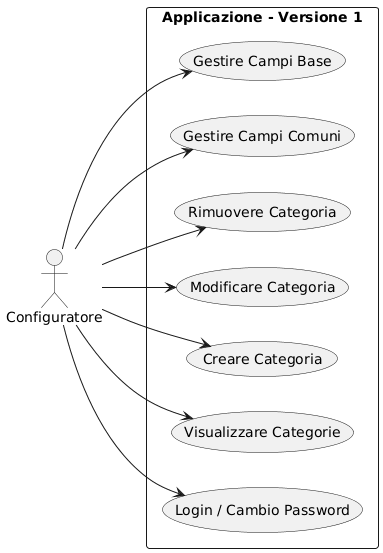
\includegraphics[width=0.8\textwidth]{../uml/casi_uso_V1.png}
    \caption{Diagramma dei Casi d'Uso - Versione 1}
    \label{fig:uc_v1}
\end{figure}

\section{Architettura e Design}

Il pattern architetturale adottato separa nettamente i dati (package \texttt{model}) dalla logica di business (package \texttt{controller}) e dalla presentazione (package \texttt{view}).

\subsection{Classi Principali (V1)}
\begin{itemize}
    \item \textbf{\texttt{Utente}} (abstract): base per tutti gli attori del sistema.
    \item \textbf{\texttt{Configuratore}} extends \texttt{Utente}: unico attore in V1.
    \item \textbf{\texttt{Categoria}}: struttura ad albero (lista di sottocategorie), contiene una mappa di \texttt{Campo}.
    \item \textbf{\texttt{Campo}}: nome, descrizione, tipo (\texttt{TipoCampo}: STRINGA, INTERO, BOOLEANO, DATA, ORA), flag obbligatorio.
    \item \textbf{\texttt{GestoreCategorie}}: logica di creazione, modifica e navigazione dell'albero.
    \item \textbf{\texttt{GestoreSessione}}: gestione login, logout e stato sessione corrente.
    \item \textbf{\texttt{GestoreFile}}: persistenza su file JSON (via libreria Gson).
    \item \textbf{\texttt{MainCLI}}: interfaccia a riga di comando; delega tutta la logica ai controller.
\end{itemize}

\subsection{Diagramma delle Classi}
Il file sorgente PlantUML è \texttt{v1\_diagramma\_classi.puml}.
\begin{figure}[h]
    \centering
    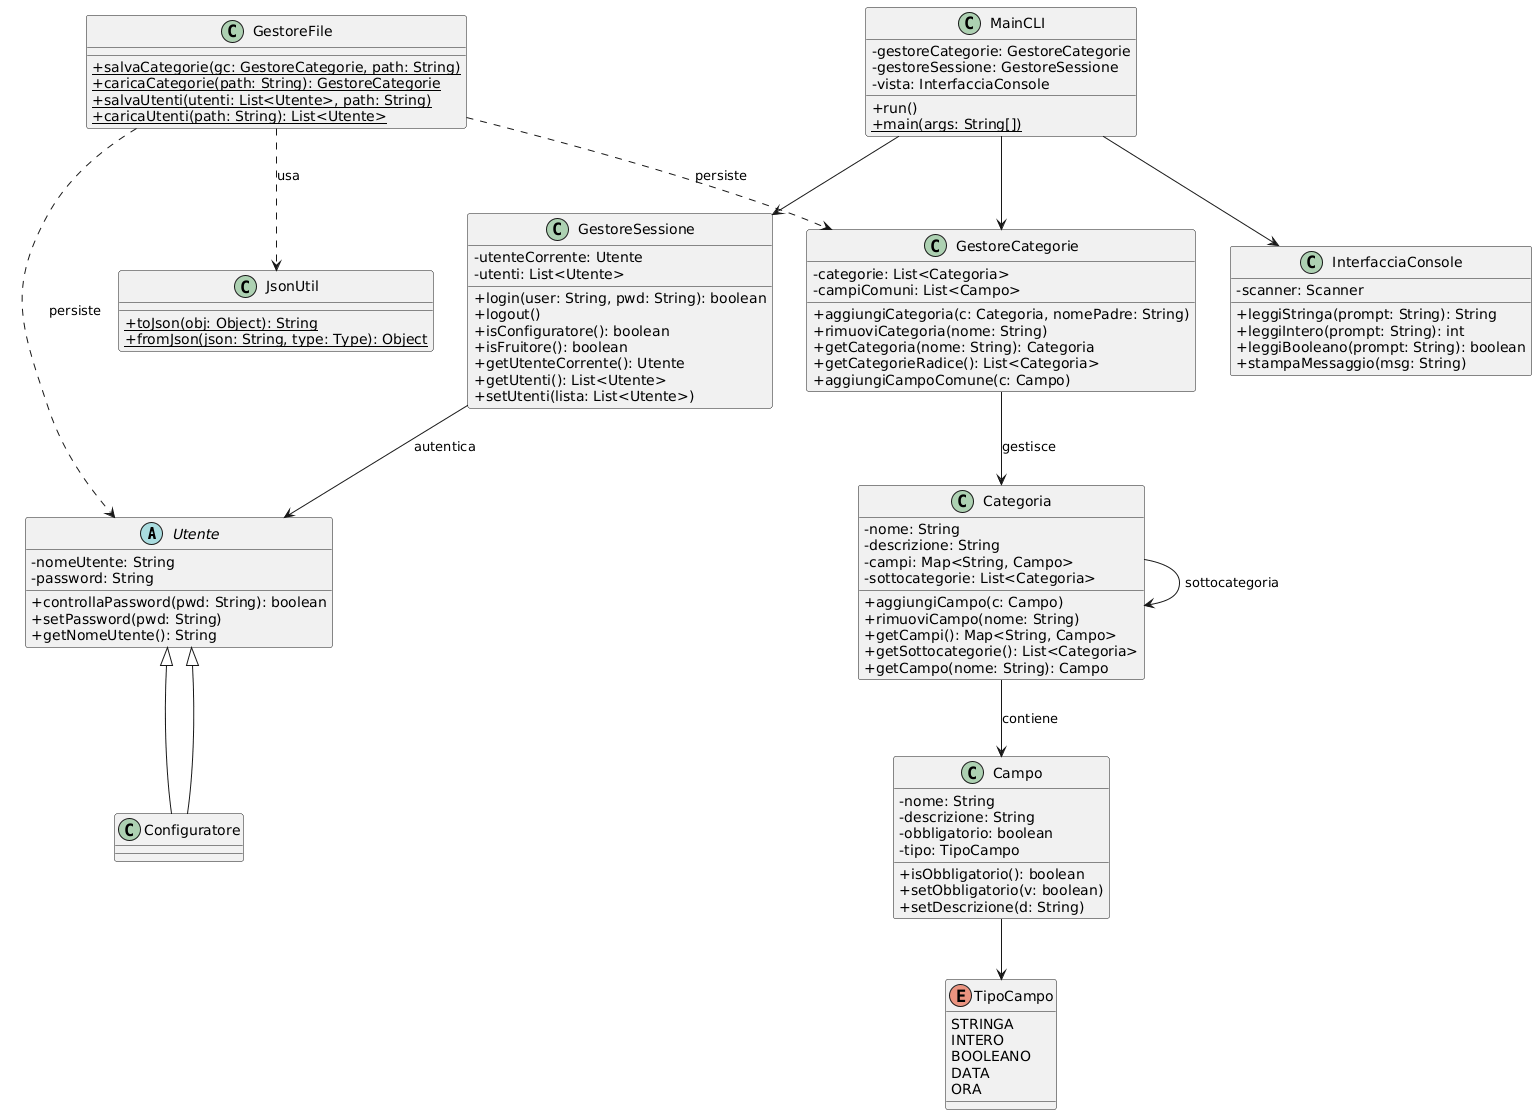
\includegraphics[width=1\textwidth]{../uml/uml_V1.png}
    \caption{Diagramma delle Classi - Versione 1}
    \label{fig:class_v1}
\end{figure}
